\documentclass[sigconf]{acmart}

\usepackage{booktabs} % For formal tables
\usepackage{array,multirow}
% Copyright
%\setcopyright{none}
%\setcopyright{acmcopyright}
%\setcopyright{acmlicensed}
\setcopyright{rightsretained}
%\setcopyright{usgov}
%\setcopyright{usgovmixed}
%\setcopyright{cagov}
%\setcopyright{cagovmixed}


% DOI
\acmDOI{10.475/123_4}

% ISBN
\acmISBN{123-4567-24-567/08/06}

%Conference
\acmConference[WOODSTOCK'97]{ACM Woodstock conference}{July 1997}{El Paso, Texas USA} 
\acmYear{1997}
%\copyrightyear{2016}


%\acmArticle{4}
%\acmPrice{15.00}

% These commands are optional
%\acmBooktitle{Transactions of the ACM Woodstock conference}
%\editor{Jennifer B. Sartor}
%\editor{Theo D'Hondt}
%\editor{Wolfgang De Meuter}


\begin{document}
%\title{Detecting Emergency Situations Based on Locations in Twitter}
\title{Self-Organized Citizen Sensors for Detecting Emergency Situations in Twitter}
\titlenote{Produces the permission block, and
  copyright information}
%\subtitle{Extended Abstract}
%\subtitlenote{The full version of the author's guide is available as
  %\texttt{acmart.pdf} document}


\author{Hernan Sarmiento}
%\authornote{Dr.~Trovato insisted his name be first.}
%\orcid{1234-5678-9012}
\affiliation{%
  \institution{Deparment of Computer Science, University of Chile}
  \streetaddress{P.O. Box 1212}
   \city{Santiago} 
   \country{Chile}}
\email{hsarmien@dcc.uchile.cl}

\author{Barbara Poblete}
%\authornote{The secretary disavows any knowledge of this author's actions.}
\affiliation{%
  \institution{Deparment of Computer Science, University of Chile}
  \streetaddress{P.O. Box 1212}
   \city{Santiago} 
   \country{Chile}}
\email{bpoblete@dcc.uchile.cl}

\author{Sergio Campos}
%\authornote{This author is the
 % one who did all the really hard work.}
\affiliation{%
  \institution{Department of Geophysics, University of Chile}
  \streetaddress{1 Th{\o}rv{\"a}ld Circle}
  \city{Santiago} 
  \country{Chile}}
\email{jaime@dgf.uchile.cl}



% The default list of authors is too long for headers.
%\renewcommand{\shortauthors}{B. Trovato et al.}


\begin{abstract}
%Most methods to detect emergency situations using Twitter rely on keyword. The problem of keyword-based methods is the need to train in specific domains and language for different type of events, for example: earthquakes, typhoons, terrorist attacks, tornadoes, etc. Our proposal is to rather use the recurring mention of a country locations in microblogging messages to identify such events without using keywords and characterize through of interarrival time probability distributions. Our method use a SVM classifier that is independent of the text language of the messages and can be training and testing among different languages and domains.

Most methods to detect emergency situations using Twitter rely on keyword. The problem of keyword-based methods is the need to train models in specific domains, in multiple languages, and for different types of events, for example: earthquakes, terrorist attacks, floods, etc. In contrast, our proposal is to rather use the recurring references of a location in the metadata of microblogging messages, where users act self-organized citizen sensors in real-locations. In order to identify an emergency situation, we characterize  such events  through frequencies, and probability distributions of the interarrival time of the messages. Our method uses a SVM classifier which is independent of the language of the text, and textual features. Finally, we describe an emergency situation according to geographic impact based on the propagation of the messages in social media between neighboring locations.
\end{abstract}




%
% The code below should be generated by the tool at
% http://dl.acm.org/ccs.cfm
% Please copy and paste the code instead of the example below. 
%
\begin{CCSXML}
	<ccs2012>
	<concept>
	<concept_id>10002951.10003227.10003236.10003239</concept_id>
	<concept_desc>Information systems~Data streaming</concept_desc>
	<concept_significance>500</concept_significance>
	</concept>
	</ccs2012>
\end{CCSXML}

\ccsdesc[500]{Information systems~Data streaming}

\keywords{Emergency Situations, Citizen Sensors, Social Media}


\maketitle

\section{Introduction}
Social media has become a major channel for communication during high-impact real-world events, for example: elections, sports events, emergency situations, etc. In any case, users act as ``citizen sensors'' where they share and post their mood, opinions, photos, videos and geographical point of interest (POI).

During emergency situations, traditional media suffer structural damage and real-time communications could be disrupted. Instead, microblogging has played a critical role in the last fifteen years since it has allowed users share real-time information from people local to the incident as current status, casualties, damages and alerts \cite{kumar2011tweettracker,imran2013extracting,stowe2016identifying,reuterfifteen}. For this reason, researchers have studied the behaviour during these events for to detect, summarize and classifyng messages with the goal to help authorities and the general public with situational awareness to act fast and conscientiously during a crisis situations.

Twitter, a microblogging which allows to share short messages (called \textit{tweets}) and is currently used world-wide by over $300$ million users\footnote{http://www.statista.com/statistics/282087/number-of-monthly-active-twitter-users/}. About $80\%$ of Twitter users access from mobile services which contribute to the inmediacy of diffusion of information specially during a crisis situations \cite{castillo2016big}. One of the main tasks during these situations is to detect a new real-event because as with most social media conversations, messages are often overcomed by irrelevant and redundant noise. In current works \cite{kumar2011tweettracker,caragea2011classifying,ashktorab2014tweedr,imranaidr2014,maldonado2017}, these tasks are solved with methods rely on keywords over \textit{Twitter Public Streaming API}\footnote{https://developer.twitter.com/en/docs/tweets/filter-realtime/overview}. The problem with these keyword-based methods is the need to train in specific domains for different type of events. \cite{olteanu2014} generate set of keywords with different datasets but sometimes arise specific terms for one event, for example \textit{\#eqnz} for Earthquake in New Zealand or \textit{\#pabloph} for Typhoon Pablo in Philippines \cite{potts2011tweeting,bruns2012local,karimi2013classifying}. Furthermore, these set of keywords are trained for a unique language and can not be used in others.

Additionally, several works related to crisis situations show a strong relationship between type of event (what) and the spatiotemporal dimensions (when and where). For example, we can see top trends during an earthquake related to locations \cite{mendoza2010twitter}, strong relationship between proximity to hurricane path and hurricane-related social media activity \cite{kryvasheyeu2016rapid}, extraction of locations and POI during floods \cite{lingad2013location} and mixing geographic information system (GIS) with geo-tagged message to improve disaster maping and real-time event tracking \cite{huang2015disastermapper}.

Based on previous works, the question we address here is: \textit{Is there evidence to detect an emergency situation based on anomaly frequency of messages that contain locations?}.

Here, we propose a method based on recurring references of country locations in message's metadata. For this task, we create a gazetteer tree based on the hierarchy of the specific country, divide the messages into fixed time-windows and compute the frequency, and the probability distributions of the inter-arrival time of the messages for each geographical hierarchy. To detect an emergency situation, we train a SVM classifier by each hierarchy and apply a geographic spread to filter false positives detection considering that an emergency situation can be \textit{Focalized} or \textit{Diffused}.  

Our main contribution is to create a methodology that detecting instantaneous emergency situations just using the locations for a specific country. Furthermore, our classifier do not depend of the language to detect a new event since that do not use textual features as input. Moreover, we characterize crisis situations that affect a small or large geographic area.

The paper is organized as follows: we first introduce an overview of relevant literature related to emergency situation and event detection in social media. Next we present a complete description of our proposal divide in four parts. Thereafter, we provide a full description of our dataset and later we summarize our experimental validation and results over the ground truth and online evaluation. Finally, we deliver our discusions, conclusions and future work.



\section{Related Work}
explain first works since 15 years ago
\subsection{Emergency Situation}
\subsubsection{Data Characterization}
crisis lex, information nuggets, twitter under crisis, disaster related messages, practical extrac-
tion of disaster-relevant, Identifying and Categorizing Disaster-Related Tweets,Microblogging
During Two Natural Hazards Events: What Twitter May Contribute to Situational Aware-
ness, Twitter Adoption and Use in Mass Convergence and Emergency Events, Twitter Under
Crisis: Can we trust what we RT?

\subsubsection{Crisis-Related Social Media Monitoring}
tweedr, twicalli, ESA, aidr, twincident, EMERSE, twicalli, tweettracker, twittris

\subsection{Event Detection}
burst detection (jheser), geo-spatial event detection, prediction and characterization of high-
activity events,Emerging event detection in social networks with location sensitivity

\subsection{Location Extraction}
pinpointing, from the justin beiber’s heart, where in the world are you?

\section{Proposed Approach}

In order to provide a complete coverage of location-based detection of emergency situation, we proposed our approach which has four stages. The following information provides details of each stage.

\subsection{Data Pre-Processing}
%In this stage, data is pre-processed from Twitter Streaming API\footnote{algo}, which allows access to subsets equal to $1\%$ of public status descriptions in real-time. With this tool, we can be retrieve messages using a set of keywords or messages from specific locations setting a bounding box. In our approach, we get entire subsets of messages without use keywords or specific locations. Then, we retrieve random messages about any topic and any place in the world.

%To increase the number of messages related to locations, we consider tweets and retweets messages. 
Since that we consider users as citizen sensors, we filter messages depending of native language of each country using the attribute \textit{lang} retrieved from Tweet Metadata\footnote{https://developer.twitter.com/en/docs/tweets/data-dictionary/overview/tweet-object}. For example, if we analyze England, we just consider messages in english. Finally, we remove user mentions, urls,  special characters and apply text tokenization . In this case, we do not remove hashtags or stopwords because some locations can be included in hashtags terms and some places can be contained stopword that can differentiate them from other similar non-related location terms.


\subsection{Signals Creation}
The problems that we address in this stage is how to infer locations from micro-blog messages to track signal over time in the Stream and what is the lowest hierarchy level to find and assign to this signal.

\subsubsection{Geographical Hierarchy}\label{sssec:geohie}
Using the idea of \textit{Gazetteer as a Tree} presented in \cite{yin2014pinpointing} in which each place is associated with a canonical taxonomy node, we construct our gazetteer tree based on Geonames\footnote{http://download.geonames.org/export/dump/} and Wikipedia\footnote{http://www.wikipedia.org/} for each country to analyze. However, in \cite{yin2014pinpointing} the gazetteer hierarchy presents four-levels where the lowest level represents a specific POIs. In our approach, we use a subset of the gazetteer hierarchy with three-levels, in which the lowest level is represented by City since a large amount of users specify their location down to the city scale \cite{hecht2011tweets}. For example, if we have the \textit{city:Manchester}, we associate this location with \textit{region-state:North West} and also with \textit{country:England}. Furthermore, the name of locations are considered just in the native language of the country. For instance, in the case of Italy locations, we consider \textit{Roma} and not \textit{Rome}.

\subsubsection{Finding Locations in Micro-Blog Metadata}

The structure of the Tweet Metadata allows to obtain information about the message and the user who shares a message. Considering the geographical hierarchy explained in the previous section, we search these locations on different levels of metadata and create one-signal for each as following:

\begin{itemize}
	\item Tweet Text: location is mentioned in the attribute \texttt{text} of tweet object, that is, on the body of the message.
	\item User Location: location is mentioned in the attribute \texttt{location} inside the \texttt{user object}, that is, the location set by the user in his profile.
	\item Tweet Text - User Location: location is mentioned in the attribute \texttt{text} of tweet object and also location is mentioned in the attribute \texttt{location} inside the \texttt{user object}. This means that the location is mentioned on the body on the message and the user who share message has the same location in his profile. In this case, tweet text and user location can be different in the smallest hierarchy but in the highest level can be equal. 
\end{itemize}

In this way, mixing geographical hierarchy and locations in micro-blog metadata, we create $NxM$ signals where $N$ is the number of locations obtained by gazetteer tree and $M$ is the number of metadata-level extracted from Tweet Object. In instance, we create a signal for \textit{city:Manchester} and we find this hierarchy in \textit{metadata:Tweet Text} and also in \textit{metadata:User Location}. That means that we track the mention of \textit{city:Manchester} at the level of the body of message and at the level of the location of the user profile individually.

\subsection{Time-Windows}
In this stage we address the problems of how to divide and determine the time-windows size to detect a new emergency situation and what variables by time-window allow it.

\subsubsection{Determining optimal window size}

According to \cite{guzman2013line}: ``If the window size is to small, the ocurrence of empty windows for a term increases, making the noise rate increate and frequency rate tend to zero. On the other hand, if the window size is too large, the stability of the signal becomes constant and busrty keyword detection is delayed''. Using this definition, we divide our signals into windows of six minutes because it divides a 24-hour day exactly, making the analysis easier to understand and to compare from different days.


\subsubsection{Normalized Frequency}
We compute the number of the messages of each time-window by signal. To normalize frequency, we compute \textit{z-score} as following:

\begin{equation} \label{eq:1}
zscore = \frac{x_{i} - \mu_{k} }{\sigma_{k}}
\end{equation}

where $x_{i}$ is the frequency of the current $i$ time-window, $\mu_{k}$ and  $\sigma_{k}$ are mean and standard deviation of the previous $k$ time-windows respectively.

%\begin{itemize}
%	\item We calculate the number of messages of each time windows for each signal.
%	\item In our first approach, we compute max-min normalization and z-score normalization of all time windows for each signal. This approach is wrong because we do not know the next values in the streaming. We just know the previous values.
%	\item We compute the z-score normalization using past values for each signal independently. We do not use rolling/moving z-score because some signals have Null values of frequency. It is happen in smallest cities or states.
%\end{itemize}
\subsubsection{Inter-arrival Time}

To characterize the urgency of the messages during a time-window, we use our previous results \cite{DBLP:conf/fdia/Sarmiento17} to compute the \textit{Inter-arrival Time} which is defined as $d_{i} = t_{i+1} - t_{i}$, where $d_{i}$ denotes the difference between two consecutive social media messages $i$ and $i+1$ that arrived in moments $t_{i}$ and $t_{i+1}$ respectively. Using this definition and according to \cite{kalyanam2016prediction}, high-activity events have a high-frequency in the first bins represented by values $d_{i} \approx 0$. 

In order to quantify a high-frequency in very small values of $d_{i}$, we compute the measures \textit{Skewness} and \textit{Kurtosis}, which represent the asymmetry and the tailedness of the shape of probability distribution respectively \cite{mardia1970measures}. Finally, we apply the equation \ref{eq:1} over \textit{Skewness} and \textit{Kurtosis} to calculate variation based on previous values.

%\begin{itemize}
%	\item Inter-arrival time represent the difference between 2 consecutive messages for one signal. In this case, a small difference between a set of messages represent the urgency or relevancy in a specific time (reference to plosone paper)
%	\item First, we compute inter-arrival time for each time windows independently. We summary results using quantiles, mean, min and max values. The problem with this approach is that we can not compare values between signals because each signal has different frequencies and behaviours along the time.
%	\item We compute skewness and kurtosis which represent a measure of the asymetry and "taildness" of the probability distribution respectively. In both case, we calculate the measures using previous values such as z-score normalization.
%\end{itemize}

%\subsection{Subsetting Signals}
%\begin{itemize}
%	\item Several signals have a null values along the time. For example, any city that is not a big city or capital city, does not a continuous frequency. To avoid this behaviour, we use cities just for compute the state frequency signal and later we discard them. Finally, we just monitor states and country hierarchy.
%	\item Furthermore, we remove gps signal because just 1-3 percent of messages have gps activated.
%\end{itemize}

\subsection{Geographic Spread}\label{sssec:geospread}

An emergency situation that affects and mobilizes response in a small area is defined as \textit{Focalized}, while a disaster with a large geographic impact is defined as \textit{Diffused} \cite{olteanu2015expect}. Using this definition, we extend this concept to represent neighborhoods between regions/states obtained from section \ref{sssec:geohie}. For that purpose, we create an \textit{Adjancency Matrix} $M$, where $M_{i,j} = 1$ represents if two states/regions are geographically connected and $M_{i,j} = 0$ if they are not connected. For instance, if an event is diffused (eg. earthquake), the detection should be in adjacent-locations independentely of metadata-level. In the other hand, if an event is focalized (eg. terrorist attack), just one-location should be detected but in different metadata-levels simultaneously.


\begin{table}
	\caption{List of earthquakes studied as ground truth, sorted by date.}
	\label{tab:eqs}
	\begin{tabular}{lccl}
		\toprule
		Country&Datetime (UTC)&Magnitude (Mw)& Language\\
		\midrule
		Italy & 2016-10-26 17:10:36 & 5.5 & Italian \\
		Italy & 2016-10-30 06:40:17 & 6.6 & Italian\\
		Chile & 2016-12-25 14:22:26 & 7.6 & Spanish\\
		Chile & 2017-04-23 02:36:06 & 5.9 & Spanish\\
		Chile & 2017-04-24 21:38:28 & 6.9 & Spanish\\
		\midrule
		%\bottomrule
	\end{tabular}
\end{table}

\section{Dataset}

In this section, data is collected from Twitter Public Streaming API, which allows access to subsets equal to $1\%$ of public status descriptions in real-time. With this tool, we can be retrieve either messages using a set of keywords or messages from specific locations setting a bounding box. In our approach, we get entire subsets of messages without use keywords or specific locations. Then, we retrieve random messages about any topic and any place in the world.
 
\subsection{Ground Truth}

We analyze five earthquakes with magnitudes between $5.5Mw$ and $7.6Mw$\footnote{Mw: the moment magnitude scale}, ocurring in Italian-speaking and Spanish-speaking countries between October 2016 and April 2017 (Table \ref{tab:eqs}). For that purpose, we collect $20$ millions of messages 12-hour before and after the emergency situation events. 

According our proposal, we create both the gazetteer hierarchies\footnote{http://users.dcc.uchile.cl/$\sim$hsarmien/gazetteer.html} for each country and construct the signals based on each hierarchy and metadata-level. As a result of the number of messages of each signal (Table \ref{tab:message_signal}), we discard all signals related to city hierarchy since a great amount of small cities have zero frequency in a normal situation unlike to capital or metropolitan cities.




\begin{table}
	\caption{Number of messages by signal.}
	\label{tab:message_signal}
	\begin{tabular}{ccl}
		\toprule
		Hierarchy&Metadata-level&Messages\\
		\midrule
		All & All & 87,291 \\
		\midrule
	    \multirow{3}{*}{Country} & Tweet Text & 11,584 \\
	    & User Location & 25,313\\
	    & Tweet Text - User Location & 1,417\\	
		\bottomrule
		\multirow{3}{*}{State} & Tweet Text & 4,110 \\
		& User Location & 13,352\\
		& Tweet Text - User Location & 86\\
		\midrule
		\multirow{3}{*}{City} & Tweet Text & 1,415 \\
		& User Location & 8,971\\
		& Tweet Text - User Location & 20\\
		\bottomrule
	\end{tabular}
\end{table} 

\subsubsection{Labeled Emergency Situations}

The exactly datetime event is obtained from National Seismology Agency in Chile\footnote{http://www.sismologia.cl/} and 
National Institute of Geophysics and Volcanology in Italy\footnote{http://www.ingv.it/it/}. For to label a time-window as \texttt{detection} class, we set detection label in those time-windows with positive variation in frequency, skewness and kurtosis respect to the normalization of the previous values (Figure \ref{fig:labeled}). Moreover, we include the three next time-windows after the event occurred to compensate the imbalance between classes.

\begin{figure}
	\centering
	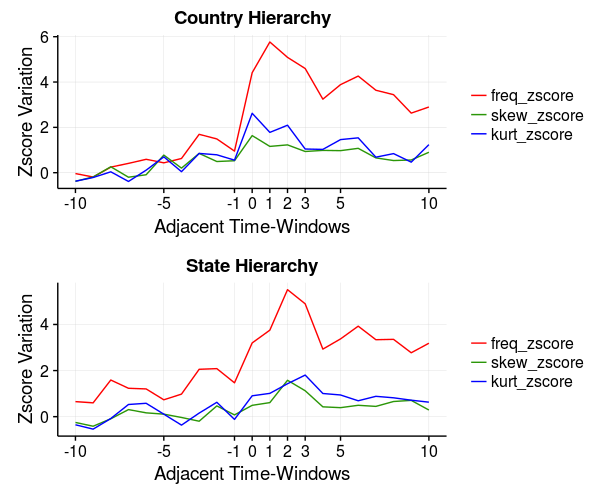
\includegraphics[width=\columnwidth]{img/labeled2.png}
	\caption{Average variation in emergency situations between time-windows.}
	\label{fig:labeled}
\end{figure}



\section{Experiments}

Our filtering task can be seen as binary classification task. The positive class (\textit{detection label}) corresponds to messages related to instantaneous emergency situations, while the negative class (\textit{nothing label}) corresponds to the remaining or non-related to crisis situations.

In order to classifier messages, we employ traditional binary classifier Support Vector Machine \textit{(SVM)}. As a result of the analyzed data scattering (Figure \ref{fig:scatter}), we separate country and state in different datasets and set both kernels and classification parameters independentely. On the one hand, \textit{country} classifier uses a polynomial kernel and strict-parameters for gamma, cost and weights since that a great amount of messages are included in country hierarchy as an effect of the minor hierarchies. On the other hand, \textit{state/region} classifier uses a linear kernel with soft-weights and cost.

\begin{figure}
	\centering
	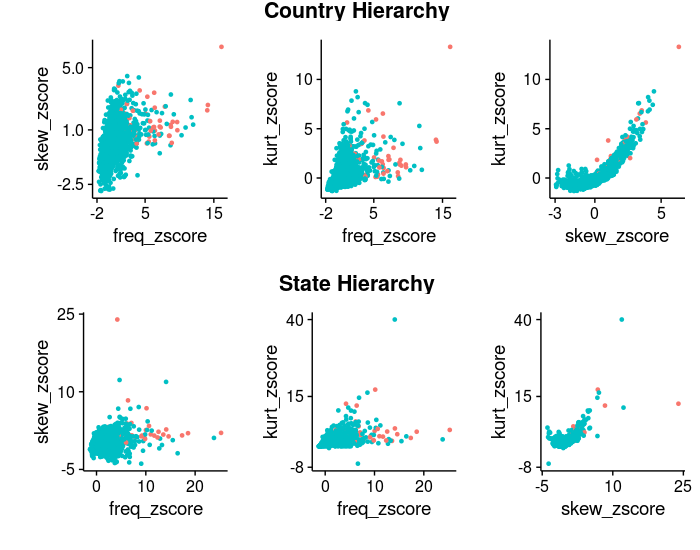
\includegraphics[width=\columnwidth]{img/scatter.png}
	\caption{Relationship between variables in country and state hierarchy. Red circles represent positive class (\textit{detection}) and blue circles represent negative class (\textit{nothing}).}
	\label{fig:scatter}
\end{figure}


Given that an emergency situation is not an usual event, we have an highly unbalanced data respect to the classes after labeled ($1\approx2\%$ of positive class corresponding to \textit{detection}). Therefore, we use \textit{under-sampling} \cite{lunardon2014rose} over country and state datasets increasing our possitive class to $15\approx18\%$. Additionally to validate our model, we use \textit{5-fold cross-validation} where one earthquake dataset is used as testing and the reamining earthquakes dataset as training.

Table \ref{tab:perfomance} shows the average results of our model applying 5-fold cross validation. In order provide a extended analysis about incorrect labels and time-windows, we include the metric \textit{False Positive Rate (FPR).} 




\subsubsection{Independent Analysis of Hierarchies} 
Our first analysis is just considering the hierarchies as isolated detections. On the top of the Table \ref{tab:perfomance}, we show the results considering only the prediction over each label in our datasets. As noted above, the assignation from the lowest level (\textit{city}) to the highest (\textit{country}) in the gazetteer hierarchy generates high frequency of messages which cause multiples \textit{bursts} in our country signal for non-related emergency situations. This concept can explain the values of Precision (\textit{P}) and \textit{FPR}.

In addition to the analysis of number of detections by labels, we also study the number of detections by time-windows. For this analysis, we search the time-windows for each hierarchy where the all metadata-level are well classified with correct class. According to the results shown on the middle of the Table \ref{tab:perfomance}, the values of Precision, F1 and FPR have worst values than the analysis by label when we analyze country and state independentely. 
\begin{table}
	\caption{Average performance of 5-fold cross-validation by hierarchy and geographic spread (G.S.)}.
	\label{tab:perfomance}
	\centering
	\begin{tabular}{c|lcccc}
		\toprule
		&Hierarchy &P &R &F1 &FPR\\
		\midrule
		\parbox[t]{2mm}{\vspace{-0.2cm}\multirow{3}{*}{\rotatebox[origin=c]{90}{\small{label}}}} 
		& Country & 0.3 & 0.83 & 0.45& 0.14\\		
		& State &0.35& 0.83& 0.5 & 0.08\\
		\midrule
		\parbox[t]{2mm}{\vspace{0cm}\multirow{5}{*}{\rotatebox[origin=c]{90}{\small{time-window}}}}
		& Country & 0.15& 0.77 & 0.25 & 0.15\\
		& State & 0.17 & 0.88 & 0.29& 0.12\\
		& Country-State& 0.35 & 0.7 & 0.47 & 0.03\\
		& Country(2)-State with G.S. & 1 & 0.64 & 0.78 & 0 \\
		& Country(3)-State with G.S. & 1 & 0.47 & 0.64 & 0\\
		\bottomrule
	\end{tabular}
\end{table}

\subsubsection{Dependent Analysis of Hierarchies}
Our second analysis is considering the hierarchies as non-isolated detections. In the results explained above, we consider country and state hierarchy independently, which is not a correct analysis because an emergency situation affect to states and country at the same time. For this reason, we inspect the time-windows where all metadata-level for country and state hierarchy have a correct detection simultaneously. The results are shown in the row \textit{Country-State} in the Table \ref{tab:perfomance}. In contrast to the independent analysis of country and state, we improve the Precision, F1 and FPR values as a consequence of a smaller amount of non-related time-windows are assigned as detection. However, when we see the value obtained for FPR ($FPR = 0.03$), this rate represents an incorrect number of time-windows assigned as detection equal to $23$. This means that we have $22$ new emergency situations detected by our classifier. 


\subsubsection{Geopraphic Spread Analysis}\label{sssec:geospreadanalysis}


Our third analysis is considering the hierarchies as non-isolated detections and using the Geographic Spread (G.S.). Using the \textit{Adjacency Matrix} to represent neighborhoods between regions/states, we consider as a correct detection those time-windows where the state/s classified as detection are defined as \textit{Focalized} or \textit{Diffused} and exist dependency between hierarchies. 
\begin{table*}
	\caption{Online evaluation by time-windows (T-W) using Country(2)-State with G.S. method}
	\label{tab:online1}
	\begin{tabular}{lclccp{3.5cm}l}
		\toprule
		Event &Detected T-W & T-W Before Event & T-W After Event & Delay(min) & Top 3 Bigrams\\
		\midrule
		Premier League Soccer Matches & 2& - & - & - & \small{(man, utd), (new, year), (happy, new)} \\
		Westminster Terrorist Attack& 13 & 0 &13 & 32& \small{(stay, safe), (terror, attack), (safe, everyone)}\\
		Manchester Terrorist Attack& 12& 1& 11& 23& \small{(ariana, grande), (incident, arena), (grande, concert)}\\
		London Terrorist Attack & 14 & 7 & 7 & 36 & \small{(stay, safe), (incident, bridge), (borough, market)}\\
		U.K. Elections& 5 & - & - & - & \small{(theresa, may), (vote, labour), (van, dijk)}\\
		Adele Live at Wembley& 9& 7&2&-& \small{(elland, road), (new, times), (phil, jackson)}\\
		England vs Eslovenia Soccer Match & 4& 4 & 0 & - & \small{(simon, brodkin), (join, us), (theresa, may)}\\
		Metallica Live at London& 4 & 4 & 0 & - & \small{(always, said), (chance, win), (carabao, cup)}\\
		\bottomrule
	\end{tabular}
\end{table*}


\begin{table*}
	\caption{Online evaluation by time-windows (T-W) using Country(3)-State with G.S. method}
	\label{tab:online2}
	\begin{tabular}{lclccp{3.5cm}l}
		\toprule
		Event &Detected T-W & T-W Before Event & T-W After Event & Delay(min) & Top 3 Bigrams\\
		\midrule
		Premier League Soccer Matches & 0& - & - & - & \hfill \break \\
		Westminster Terrorist Attack& 4 & 0 &4 & 32& \small{(terror, attack), (stay, safe), (terrorist, attack)}\\
		Manchester Terrorist Attack& 2& 0& 2& 23& \small{(ariana, grande), (praying, everyone), (everyone, affected)}\\
		London Terrorist Attack & 1 & 1 & 0 & - & \small{(ariana, grande), (around, world), (lady, gaga)} \\
		U.K. Elections& 0 & - & - & - & \hfill \break\\
		Adele Live at Wembley& 0& 0&0&-& \hfill \break\\
		England vs Eslovenia Soccer Match & 1& 1 & 0 & - & \small{(per, day), (menswear, sample), (closed, roads)}\\
		Metallica Live at London& 2 & 2 & 0 & - & \small{(happy, birthday), (chance, win), (always, said)}\\
		\bottomrule
	\end{tabular}
\end{table*}
In addition to the results of the dependency analysis explained above, we see that a large amount of time-windows ($\approx 82\%$) for country hierarchy have more than one metadata-level when exist a correct detection. This can be explained since an emergency situation produce a collective reaction on the level of body of the message (\textit{tweet text}), users sharing any messages with profile location in a specific country (\textit{user location}) or mixing both concepts (\textit{tweet text - user location}).


Considering the geographic spread by states and the number of metadata-levels by country hierarchy, we analyze the results shown on the bottom of the Table \ref{tab:perfomance}. On the one hand, the row with value equal to \textit{Country(2)-State with G.S.} represent the detection when we consider at least two metadata-levels for the country hierarchy and the geographic spread for states. In contrast to the the previous analyzes, we improve the values of the Precision, F1 and FPR. The last metrics is very important because there are not exist time-windows incorrectly assigned as emergency situations. Consequently, the Recall values decrease which means that our method remove some time-windows classified as detection. Beside the percent of emergency situations detected is equal to $100\%$ with a average delay equal to $10.4$ minutes ($min=6$, $max=14$) from the impact of the event to the detection.


On the other hand, \textit{Country(3)-State with G.S.} represent the detection when we consider three metadata-levels for country hierarchy and the geographic spread for states. Similar to  \textit{Country(2)-State with G.S.}, we improve the values of Precision, F1 and FPR but our recall decrease from $R = 0.58$ to $R = 0.47$, detecting  $80\%$ of the emergency situations with a average delay equal $11.5$ minutes ($min=8$, $max=14$) from the impact of the event to the detection.


\subsection{Online Evaluation}
For our evaluation in the Twitter Public Stream, we training our classifier with the five earthquakes identify in our ground truth. Futhermore, our evaluation dataset is formed by eight different events that ocurred in England between December 2016 and October 2017. For each event we consider the full-day in which they ocurred. The main goals of this evaluation is to know the capacity of our method to detect emergency situations and discard non-related to emergency situations that involve references of locations. Geographic spread analysis is used to evaluate our method because decrease the number of false positive detection. In the same way of the experiments in Section \ref{sssec:geospreadanalysis}, we compare the results using the two presented methods respect to the number of metadata-levels by country hierarchy.

As can be appreciated on Table \ref{tab:online1} and Table \ref{tab:online2}, we study three terrorist attacks and five high-impact real-world events related to soccer matches, music concerts and political elections. In the case of Premier League Soccer Matches and U.K Elections, we cannot identify the beginning of the event, since that in the first one there are many soccer matches during the analyzed day and in the second one there is not a specific start time. In order to know the topics when our method detect an event, we compute the Top 3 Bigrams in the detected time-windows. Also, we calculate the delay time just for emergency situations events.

On the one hand, the first evaluation \textit{Country(2)-State with G.S.} has full detection of the terrorist attacks with average delay time equal to $30.3$ minutes. These detections are related to the event given that the bigrams represent terms associated with crisis situations. However, the London Terrorist Attack has $50\%$ of the detected time-windows after the event, which means that there are seven time-windows non-related to emergency situations. Besides to the crisis situations analysis, we also study the number of detected time-windows in non-related to emergency situation events. In the same way, we have a large amount of misclassified time-windows that do not represent crisis situations as we can see in the Top 3 Bigrams for each non-related to event.

On the other hand, the second evaluation \textit{Country(3)-State with G.S.} decreases the number non-related to emergency situations detected as crisis situations. We can see three time-windows in two events detected as emergency situations (England vs Eslovenia, and Metallica Live at London). In these cases, the time-windows are detected before the event and corresponding a non-emergency situations according to the bigrams. Furthermore, when we analyzed the number of the detected emergency situations, two-third ($66\%$) of the events are detected correctly with average delay time equal to $30.3$ minutes . In the case of London Terrorist Attack, our method detects one time-window before the event but the bigrams describe that the detection do not correspond to crisis situations.

%Unlike to  \textit{Country(2)-State with G.S} method, \textit{Country(3)-State with G.S} method decreases the number of detection by time-windows given that latter is stricter than the first one respect to the number of country detection by metadata-level.


\begin{figure}
	\centering
	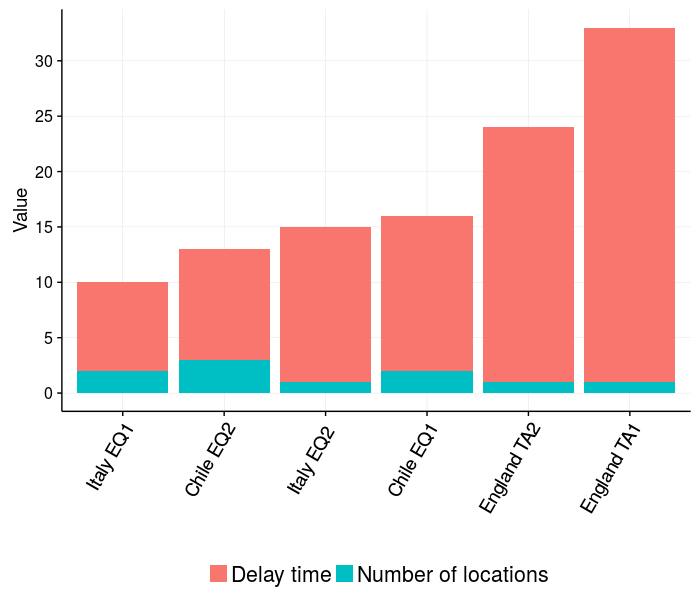
\includegraphics[width=\columnwidth]{img/delay.png}
	\caption{Delay time and number of locations in the first detection for diffused and focalized emergency situacions.}
	\label{fig:delay}
\end{figure}

\section{Discussion}

Our findings suggest that there is evidence to detect an emergency situation based on anomaly frequency of messages that contain locations for a specific country. Indeed, our method based on the number of metadata-levels by country hierarchy and geographic spread by state, detect $80\%$ of the events related to emergency situations as we could demostrate in our ground truth. Also, our method is independent of the textual features because we apply the model over different languages as spanish, italian and english. Furthermore, we test our model ind different type of events such as earthquakes and terrorist attacks
and also on different magnitudes (in the case of earthquakes) and affected people (e.g: Manchester Terrorist Attack vs Westminster Terrorist Attack).

However, when we apply our method in the online evaluation , we detect $66\%$ of the emergency situations that affected to England. This can explain because the signal are noise but many reason: the number of active users in United Kingdom\footnote{http://www.statista.com/statistics/242606/number-of-active-twitter-users-in-selected-countries/ visited on January 2018} which can affect the anomaly frequency of message since that exist a high daily average activity of the messages; similar locations in other countries (York $\approx$ New York); and soccer teams with names of cities (Manchester United, Liverpool). These issues also can affect the number of false positive detection in which in the case of England was $30\%$ of the non-related to emergency situations events.

Reggarding the geographic spread where we define an emergency situation as diffused or focalized, we find some evidences that differentiate them. In the case of diffused events, the delay time of the our first detection was less than $12$ minutes and in focalized events was greater than $30$ minutes (Figure \ref{fig:delay}). This can be explain given that, in diffused events such as earthquakes, a large amount of people are affected (thousand or millions) at the same time by an event which generate a collective reaction in social media in the locations where the event impact. In Figure \ref{fig:delay}, we can see that earthquakes have at least two detected locations in the first detection (except Italy EQ2). In contrast, focalized events have less amount of eyewitness (hundred or thousands) then when the users share messages in social media, the frequency not affect the average daily message of the country in the first minutes. This can be explain en Figure \ref{fig:delay} where the terrorist attacks have just 1 detected locations in the first detection.

Additionally, the delay time can be different according to many reason: datetime of the event (for example, during the early hours), little differences with the end of the current time-window, type of the affected locations (rural, urban cities) and the number of active users by locations.

%\begin{itemize}
%	\item explain that we dont need compute textual features as bigrams, top-k terms.
%	\item explain that we just need de gazetteer tree
%	\item explain when our methodology could be not working. eg. why not working correctly in england. country with many language. How event like soccer match are filtered and when not working
%	\item Delay time: explain difference between focalized and diffused event. People feel the event at the same time, activity in affected locations.
%	\item Number of locations affected in the first and second detection for focalized and diffused (plot)
%	\item Diffused: mercalli and locations detected.
	
%\end{itemize}

\section{Conclusion}

In this paper we have presented a methodology for detecting an emergency situation based on location for a specific country. This approach is independent of the textual features and can be used in different type of events and languages. We show that the users act self-organized in the affected locations like citizen sensors when an emergency situation occur. We furthermore have presented an analysis of geographic spread for different type of events, allowing characterize them. However, our experiment consider just a small portion of emergency situations which is not representive for all type of crisis situations according either the hazard type (natural or human-induced), temporal development (instantaneous or progressive) or geographic spread (diffused or focalized).

There are many things that can be improved our results. We will add Point of Interest to our gazetteer tree to increase the frequency by time-windows in each hierarchy. Furthermore, we will add more non-textual features as number of retweets and tweets, unique locations detected and special locations. We also plan study the relevance of the different metadata-levels and assign weights for each. Finally, we will create a web application to visualize in real-time events.

\begin{acks}
	The authors would like to thank Dr. Yuhua Li for providing the
	MATLAB code of the \textit{BEPS} method.
	
	The authors would also like to thank the anonymous referees for
	their valuable comments and helpful suggestions. The work is
	supported by the \grantsponsor{GS501100001809}{National Natural
		Science Foundation of
		China}{http://dx.doi.org/10.13039/501100001809} under Grant
	No.:~\grantnum{GS501100001809}{61273304}
	and~\grantnum[http://www.nnsf.cn/youngscientists]{GS501100001809}{Young
		Scientists' Support Program}.
	
\end{acks}

%\begin{itemize}
%	\item Add features for filtering detection: textual features. E.g: subjectivity, present tense, number of hashtag relative to the number of post, number of @s relative to the number of post, RT ratio, number of post that contain links.
%	\item Add features to classifier similar to above.
%	\item Evaluate the effect of gps signal.
%\end{itemize}


\bibliographystyle{ACM-Reference-Format}
\bibliography{bio} 

\end{document}
